\documentclass{standalone}
\usepackage{tikz}
\usetikzlibrary{patterns, positioning}


\begin{document}
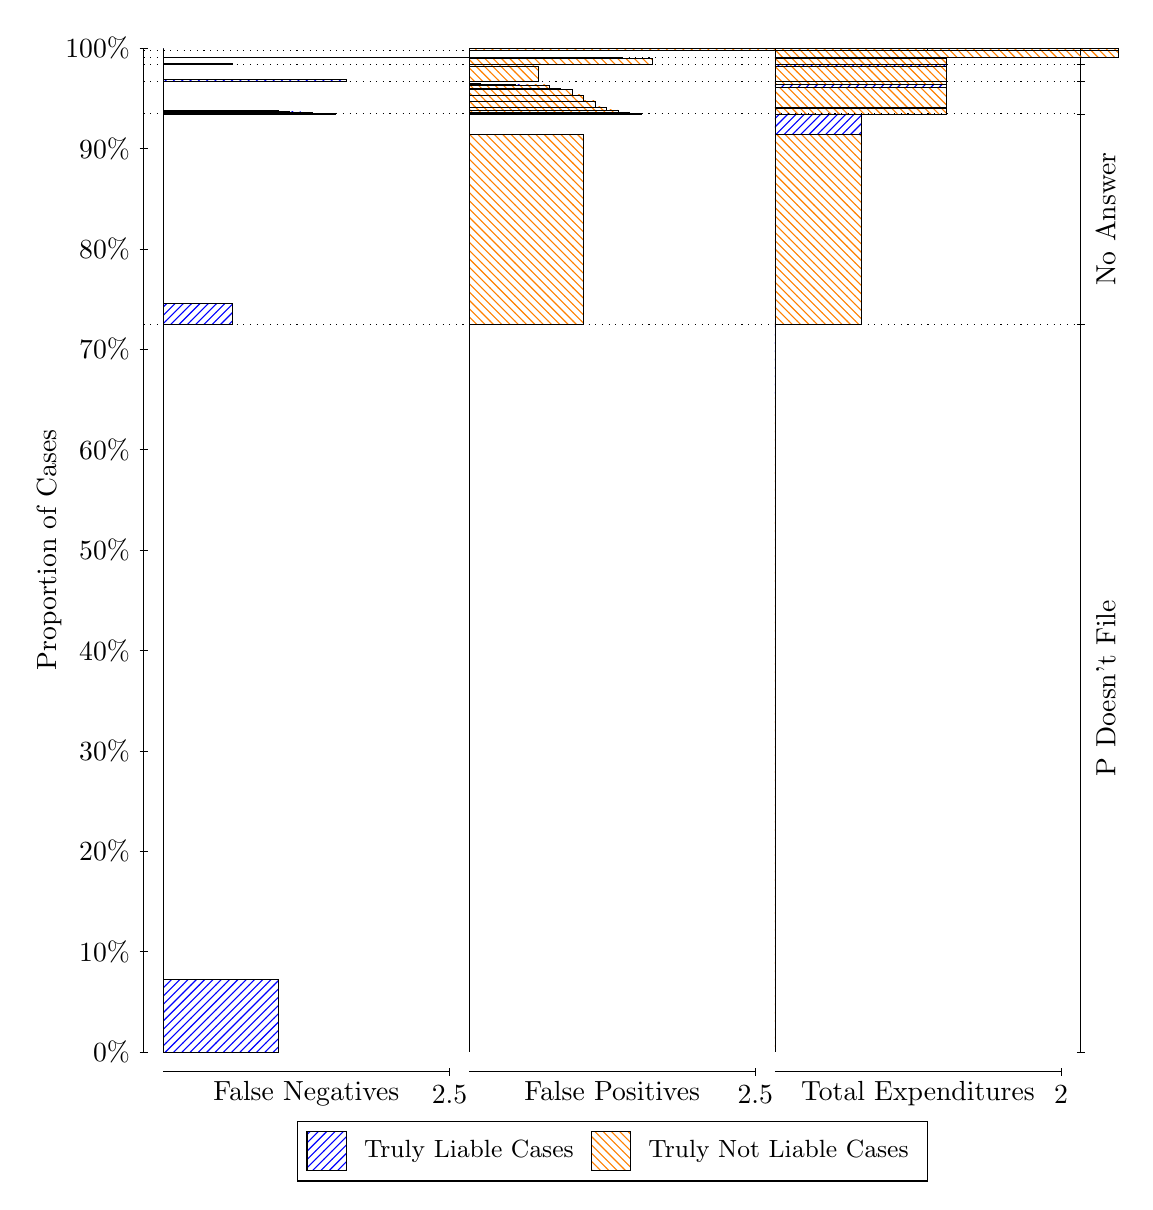
\begin{tikzpicture}
\draw[black, very thin] (1.5,1.75) -- (1.5,14.5);
\node[rotate=90, text=black, anchor=center] at (0.3, 8.125) {Proportion of Cases};
\draw[black, very thin] (1.45,1.75) -- (1.55,1.75);
\node[text=black, anchor=east] at (1.45, 1.75) {0\%};
\draw[black, very thin] (1.45,3.025) -- (1.55,3.025);
\node[text=black, anchor=east] at (1.45, 3.025) {10\%};
\draw[black, very thin] (1.45,4.3) -- (1.55,4.3);
\node[text=black, anchor=east] at (1.45, 4.3) {20\%};
\draw[black, very thin] (1.45,5.575) -- (1.55,5.575);
\node[text=black, anchor=east] at (1.45, 5.575) {30\%};
\draw[black, very thin] (1.45,6.85) -- (1.55,6.85);
\node[text=black, anchor=east] at (1.45, 6.85) {40\%};
\draw[black, very thin] (1.45,8.125) -- (1.55,8.125);
\node[text=black, anchor=east] at (1.45, 8.125) {50\%};
\draw[black, very thin] (1.45,9.4) -- (1.55,9.4);
\node[text=black, anchor=east] at (1.45, 9.4) {60\%};
\draw[black, very thin] (1.45,10.675) -- (1.55,10.675);
\node[text=black, anchor=east] at (1.45, 10.675) {70\%};
\draw[black, very thin] (1.45,11.95) -- (1.55,11.95);
\node[text=black, anchor=east] at (1.45, 11.95) {80\%};
\draw[black, very thin] (1.45,13.225) -- (1.55,13.225);
\node[text=black, anchor=east] at (1.45, 13.225) {90\%};
\draw[black, very thin] (1.45,14.5) -- (1.55,14.5);
\node[text=black, anchor=east] at (1.45, 14.5) {100\%};

\draw[black, very thin] (13.4,1.75) -- (13.4,14.5);
\draw[black, very thin] (13.35,1.75) -- (13.45,1.75);
\node[anchor=west] at (13.35, 1.75) {};
\draw[black, very thin] (13.35,10.992) -- (13.45,10.992);
\node[anchor=west] at (13.35, 10.992) {};
\draw[black, very thin] (13.35,13.663) -- (13.45,13.663);
\node[anchor=west] at (13.35, 13.663) {};
\draw[black, very thin] (13.35,14.079) -- (13.45,14.079);
\node[anchor=west] at (13.35, 14.079) {};
\draw[black, very thin] (13.35,14.292) -- (13.45,14.292);
\node[anchor=west] at (13.35, 14.292) {};
\draw[black, very thin] (13.35,14.383) -- (13.45,14.383);
\node[anchor=west] at (13.35, 14.383) {};
\draw[black, very thin] (13.35,14.473) -- (13.45,14.473);
\node[anchor=west] at (13.35, 14.473) {};
\draw[black, very thin] (13.35,14.5) -- (13.45,14.5);
\node[anchor=west] at (13.35, 14.5) {};

\draw[black, very thin, pattern color=blue, pattern=north east lines] (1.75,1.75) rectangle (3.2033,2.6742);
\draw[black, very thin, pattern color=orange, pattern=north west lines] (1.75,2.6742) rectangle (1.75,10.992);
\draw[black, very thin, pattern color=blue, pattern=north east lines] (1.75,10.992) rectangle (2.622,11.254);
\draw[black, very thin, pattern color=orange, pattern=north west lines] (1.75,11.254) rectangle (1.75,13.663);
\draw[black, very thin, pattern color=blue, pattern=north east lines] (1.75,13.663) rectangle (3.93,13.666);
\draw[black, very thin, pattern color=blue, pattern=north east lines] (1.75,13.666) rectangle (3.7847,13.669);
\draw[black, very thin, pattern color=blue, pattern=north east lines] (1.75,13.669) rectangle (3.6393,13.678);
\draw[black, very thin, pattern color=blue, pattern=north east lines] (1.75,13.678) rectangle (3.494,13.688);
\draw[black, very thin, pattern color=blue, pattern=north east lines] (1.75,13.688) rectangle (3.3487,13.699);
\draw[black, very thin, pattern color=blue, pattern=north east lines] (1.75,13.699) rectangle (3.2033,13.704);
\draw[black, very thin, pattern color=blue, pattern=north east lines] (1.75,13.704) rectangle (3.058,13.707);
\draw[black, very thin, pattern color=blue, pattern=north east lines] (1.75,13.707) rectangle (2.9127,13.709);
\draw[black, very thin, pattern color=blue, pattern=north east lines] (1.75,13.709) rectangle (2.7673,13.711);
\draw[black, very thin, pattern color=orange, pattern=north west lines] (1.75,13.711) rectangle (1.75,14.079);
\draw[black, very thin, pattern color=blue, pattern=north east lines] (1.75,14.079) rectangle (4.0753,14.097);
\draw[black, very thin, pattern color=orange, pattern=north west lines] (1.75,14.097) rectangle (1.75,14.292);
\draw[black, very thin, pattern color=blue, pattern=north east lines] (1.75,14.292) rectangle (2.622,14.305);
\draw[black, very thin, pattern color=orange, pattern=north west lines] (1.75,14.305) rectangle (1.75,14.383);
\draw[black, very thin, pattern color=blue, pattern=north east lines] (1.75,14.383) rectangle (7.5633,14.385);
\draw[black, very thin, pattern color=orange, pattern=north west lines] (1.75,14.385) rectangle (1.75,14.473);
\draw[black, very thin, pattern color=orange, pattern=north west lines] (1.75,14.473) rectangle (1.75,14.492);
\draw[black, very thin, pattern color=blue, pattern=north east lines] (1.75,14.492) rectangle (1.75,14.5);
\draw[black, very thin, pattern color=orange, pattern=north west lines] (5.6333,1.75) rectangle (5.6333,10.068);
\draw[black, very thin, pattern color=blue, pattern=north east lines] (5.6333,10.068) rectangle (5.6333,10.992);
\draw[black, very thin, pattern color=orange, pattern=north west lines] (5.6333,10.992) rectangle (7.0867,13.4);
\draw[black, very thin, pattern color=blue, pattern=north east lines] (5.6333,13.4) rectangle (5.6333,13.663);
\draw[black, very thin, pattern color=orange, pattern=north west lines] (5.6333,13.663) rectangle (7.8133,13.674);
\draw[black, very thin, pattern color=orange, pattern=north west lines] (5.6333,13.674) rectangle (7.668,13.685);
\draw[black, very thin, pattern color=orange, pattern=north west lines] (5.6333,13.685) rectangle (7.5227,13.713);
\draw[black, very thin, pattern color=orange, pattern=north west lines] (5.6333,13.713) rectangle (7.3773,13.753);
\draw[black, very thin, pattern color=orange, pattern=north west lines] (5.6333,13.753) rectangle (7.232,13.83);
\draw[black, very thin, pattern color=orange, pattern=north west lines] (5.6333,13.83) rectangle (7.0867,13.906);
\draw[black, very thin, pattern color=orange, pattern=north west lines] (5.6333,13.906) rectangle (6.9413,13.972);
\draw[black, very thin, pattern color=orange, pattern=north west lines] (5.6333,13.972) rectangle (6.796,13.988);
\draw[black, very thin, pattern color=orange, pattern=north west lines] (5.6333,13.988) rectangle (6.6507,14.031);
\draw[black, very thin, pattern color=blue, pattern=north east lines] (5.6333,14.031) rectangle (6.36,14.033);
\draw[black, very thin, pattern color=blue, pattern=north east lines] (5.6333,14.033) rectangle (6.2147,14.034);
\draw[black, very thin, pattern color=blue, pattern=north east lines] (5.6333,14.034) rectangle (6.0693,14.038);
\draw[black, very thin, pattern color=blue, pattern=north east lines] (5.6333,14.038) rectangle (5.924,14.043);
\draw[black, very thin, pattern color=blue, pattern=north east lines] (5.6333,14.043) rectangle (5.7787,14.053);
\draw[black, very thin, pattern color=blue, pattern=north east lines] (5.6333,14.053) rectangle (5.6333,14.079);
\draw[black, very thin, pattern color=orange, pattern=north west lines] (5.6333,14.079) rectangle (6.5053,14.274);
\draw[black, very thin, pattern color=blue, pattern=north east lines] (5.6333,14.274) rectangle (5.6333,14.292);
\draw[black, very thin, pattern color=orange, pattern=north west lines] (5.6333,14.292) rectangle (7.9587,14.37);
\draw[black, very thin, pattern color=blue, pattern=north east lines] (5.6333,14.37) rectangle (6.5053,14.383);
\draw[black, very thin, pattern color=orange, pattern=north west lines] (5.6333,14.383) rectangle (5.6333,14.471);
\draw[black, very thin, pattern color=blue, pattern=north east lines] (5.6333,14.471) rectangle (5.6333,14.473);
\draw[black, very thin, pattern color=orange, pattern=north west lines] (5.6333,14.473) rectangle (11.447,14.492);
\draw[black, very thin, pattern color=blue, pattern=north east lines] (5.6333,14.492) rectangle (9.9933,14.5);
\draw[black, very thin, pattern color=orange, pattern=north west lines] (9.5167,1.75) rectangle (9.5167,10.068);
\draw[black, very thin, pattern color=blue, pattern=north east lines] (9.5167,10.068) rectangle (9.5167,10.992);
\draw[black, very thin, pattern color=orange, pattern=north west lines] (9.5167,10.992) rectangle (10.607,13.4);
\draw[black, very thin, pattern color=blue, pattern=north east lines] (9.5167,13.4) rectangle (10.607,13.663);
\draw[black, very thin, pattern color=orange, pattern=north west lines] (9.5167,13.663) rectangle (11.697,13.74);
\draw[black, very thin, pattern color=blue, pattern=north east lines] (9.5167,13.74) rectangle (11.697,13.751);
\draw[black, very thin, pattern color=orange, pattern=north west lines] (9.5167,13.751) rectangle (11.697,14.003);
\draw[black, very thin, pattern color=blue, pattern=north east lines] (9.5167,14.003) rectangle (11.697,14.035);
\draw[black, very thin, pattern color=orange, pattern=north west lines] (9.5167,14.035) rectangle (11.697,14.074);
\draw[black, very thin, pattern color=blue, pattern=north east lines] (9.5167,14.074) rectangle (11.697,14.079);
\draw[black, very thin, pattern color=orange, pattern=north west lines] (9.5167,14.079) rectangle (11.697,14.274);
\draw[black, very thin, pattern color=blue, pattern=north east lines] (9.5167,14.274) rectangle (11.697,14.292);
\draw[black, very thin, pattern color=orange, pattern=north west lines] (9.5167,14.292) rectangle (11.697,14.37);
\draw[black, very thin, pattern color=blue, pattern=north east lines] (9.5167,14.37) rectangle (11.697,14.383);
\draw[black, very thin, pattern color=orange, pattern=north west lines] (9.5167,14.383) rectangle (13.877,14.471);
\draw[black, very thin, pattern color=blue, pattern=north east lines] (9.5167,14.471) rectangle (13.877,14.473);
\draw[black, very thin, pattern color=orange, pattern=north west lines] (9.5167,14.473) rectangle (13.877,14.492);
\draw[black, very thin, pattern color=blue, pattern=north east lines] (9.5167,14.492) rectangle (13.877,14.5);
\draw[black, dotted] (1.5,10.992) -- (13.4,10.992);
\draw[black, dotted] (1.5,13.663) -- (13.4,13.663);
\draw[black, dotted] (1.5,14.079) -- (13.4,14.079);
\draw[black, dotted] (1.5,14.292) -- (13.4,14.292);
\draw[black, dotted] (1.5,14.383) -- (13.4,14.383);
\draw[black, dotted] (1.5,14.473) -- (13.4,14.473);
\draw[black, very thin] (1.75,1.5) -- (5.3833,1.5);
\node[text=black, anchor=north] at (3.5667, 1.5) {False Negatives};
\draw[black, very thin] (5.3833,1.45) -- (5.3833,1.55);
\node[text=black, anchor=north] at (5.3833, 1.45) {2.5};

\draw[black, very thin] (5.6333,1.5) -- (9.2667,1.5);
\node[text=black, anchor=north] at (7.45, 1.5) {False Positives};
\draw[black, very thin] (9.2667,1.45) -- (9.2667,1.55);
\node[text=black, anchor=north] at (9.2667, 1.45) {2.5};

\draw[black, very thin] (9.5167,1.5) -- (13.15,1.5);
\node[text=black, anchor=north] at (11.333, 1.5) {Total Expenditures};
\draw[black, very thin] (13.15,1.45) -- (13.15,1.55);
\node[text=black, anchor=north] at (13.15, 1.45) {2};

\node[text=black, centered, rotate=90] at (13.72, 6.371) {P Doesn't File};
\node[text=black, centered, rotate=90] at (13.72, 12.327) {No Answer};






\draw (7.449999999999999,1.5) node[draw=none] (baseCoordinate) {};
\begin{scope}[align=center]
        \matrix[scale=0.5, draw=black, below=0.5cm of baseCoordinate, nodes={draw}, column sep=0.1cm]{
            \node[rectangle, draw, minimum width=0.5cm, minimum height=0.5cm, pattern color=blue, pattern=north east lines] {}; &
            \node[draw=none, font=\small, text=black] (B) {Truly Liable Cases}; &
            \node[rectangle, draw, minimum width=0.5cm, minimum height=0.5cm, pattern color=orange, pattern=north west lines] {}; &
            \node[draw=none, font=\small, text=black] (B) {Truly Not Liable Cases}; \\
            };
\end{scope}

\end{tikzpicture}
\end{document}